\documentclass{standalone}
\usepackage{tikz}
\usetikzlibrary{patterns, positioning}


\begin{document}
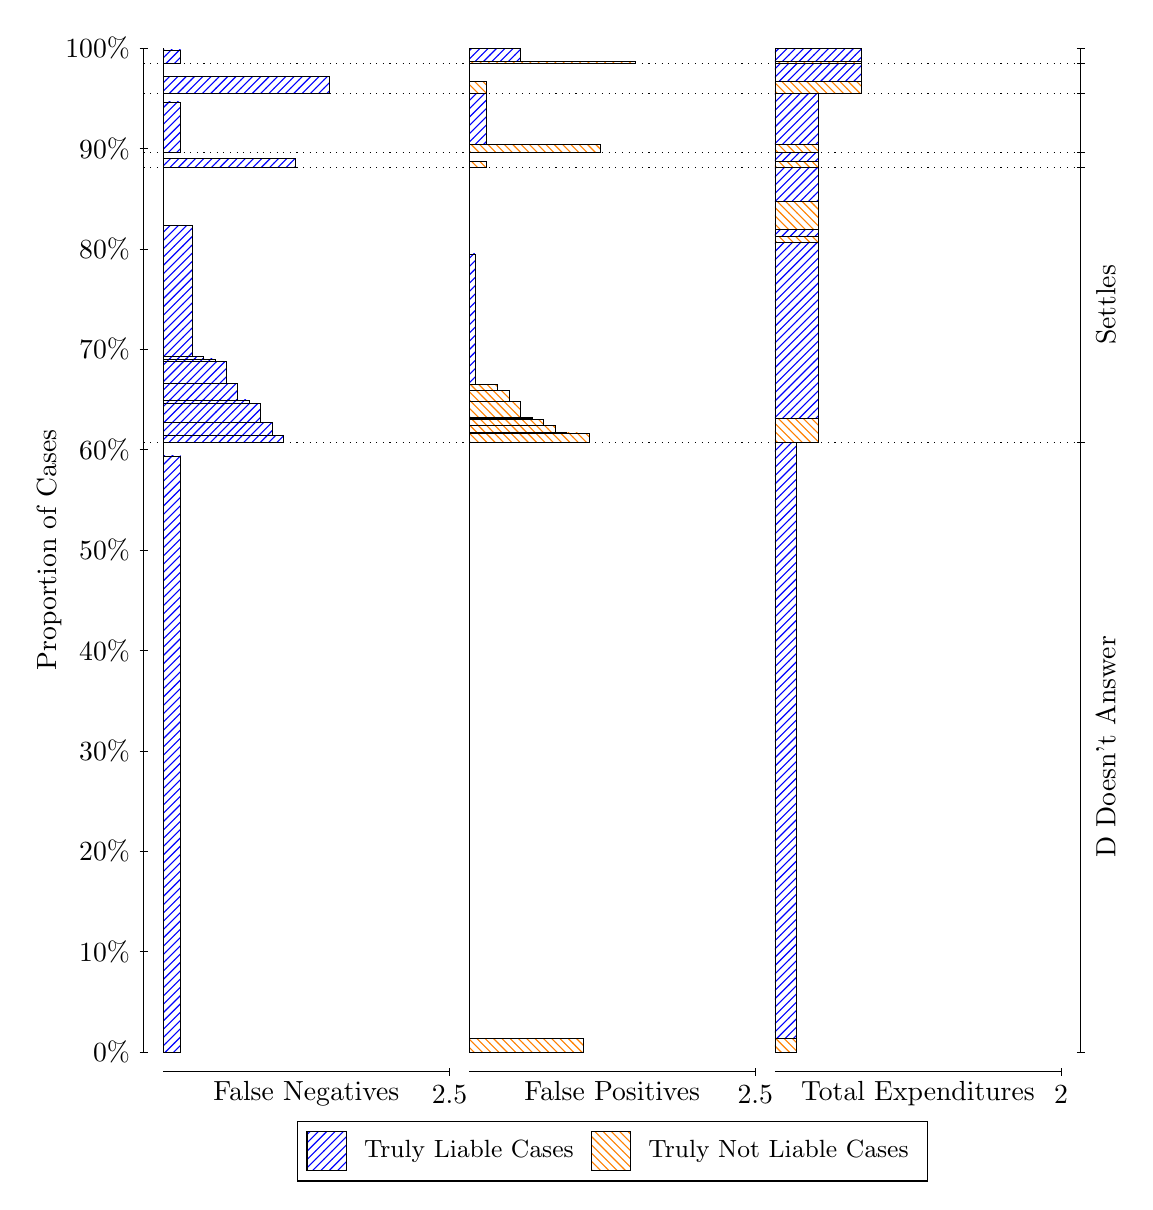
\begin{tikzpicture}
\draw[black, very thin] (1.5,1.75) -- (1.5,14.5);
\node[rotate=90, text=black, anchor=center] at (0.3, 8.125) {Proportion of Cases};
\draw[black, very thin] (1.45,1.75) -- (1.55,1.75);
\node[text=black, anchor=east] at (1.45, 1.75) {0\%};
\draw[black, very thin] (1.45,3.025) -- (1.55,3.025);
\node[text=black, anchor=east] at (1.45, 3.025) {10\%};
\draw[black, very thin] (1.45,4.3) -- (1.55,4.3);
\node[text=black, anchor=east] at (1.45, 4.3) {20\%};
\draw[black, very thin] (1.45,5.575) -- (1.55,5.575);
\node[text=black, anchor=east] at (1.45, 5.575) {30\%};
\draw[black, very thin] (1.45,6.85) -- (1.55,6.85);
\node[text=black, anchor=east] at (1.45, 6.85) {40\%};
\draw[black, very thin] (1.45,8.125) -- (1.55,8.125);
\node[text=black, anchor=east] at (1.45, 8.125) {50\%};
\draw[black, very thin] (1.45,9.4) -- (1.55,9.4);
\node[text=black, anchor=east] at (1.45, 9.4) {60\%};
\draw[black, very thin] (1.45,10.675) -- (1.55,10.675);
\node[text=black, anchor=east] at (1.45, 10.675) {70\%};
\draw[black, very thin] (1.45,11.95) -- (1.55,11.95);
\node[text=black, anchor=east] at (1.45, 11.95) {80\%};
\draw[black, very thin] (1.45,13.225) -- (1.55,13.225);
\node[text=black, anchor=east] at (1.45, 13.225) {90\%};
\draw[black, very thin] (1.45,14.5) -- (1.55,14.5);
\node[text=black, anchor=east] at (1.45, 14.5) {100\%};

\draw[black, very thin] (13.4,1.75) -- (13.4,14.5);
\draw[black, very thin] (13.35,1.75) -- (13.45,1.75);
\node[anchor=west] at (13.35, 1.75) {};
\draw[black, very thin] (13.35,9.4955) -- (13.45,9.4955);
\node[anchor=west] at (13.35, 9.4955) {};
\draw[black, very thin] (13.35,12.98) -- (13.45,12.98);
\node[anchor=west] at (13.35, 12.98) {};
\draw[black, very thin] (13.35,13.173) -- (13.45,13.173);
\node[anchor=west] at (13.35, 13.173) {};
\draw[black, very thin] (13.35,13.921) -- (13.45,13.921);
\node[anchor=west] at (13.35, 13.921) {};
\draw[black, very thin] (13.35,14.303) -- (13.45,14.303);
\node[anchor=west] at (13.35, 14.303) {};
\draw[black, very thin] (13.35,14.5) -- (13.45,14.5);
\node[anchor=west] at (13.35, 14.5) {};

\draw[black, very thin, pattern color=blue, pattern=north east lines] (1.75,1.75) rectangle (1.968,9.3206);
\draw[black, very thin, pattern color=orange, pattern=north west lines] (1.75,9.3206) rectangle (1.75,9.4955);
\draw[black, very thin, pattern color=blue, pattern=north east lines] (1.75,9.4955) rectangle (3.276,9.5806);
\draw[black, very thin, pattern color=blue, pattern=north east lines] (1.75,9.5806) rectangle (3.1307,9.7425);
\draw[black, very thin, pattern color=blue, pattern=north east lines] (1.75,9.7425) rectangle (2.9853,9.9906);
\draw[black, very thin, pattern color=blue, pattern=north east lines] (1.75,9.9906) rectangle (2.84,10.032);
\draw[black, very thin, pattern color=blue, pattern=north east lines] (1.75,10.032) rectangle (2.6947,10.245);
\draw[black, very thin, pattern color=blue, pattern=north east lines] (1.75,10.245) rectangle (2.5493,10.516);
\draw[black, very thin, pattern color=blue, pattern=north east lines] (1.75,10.516) rectangle (2.404,10.553);
\draw[black, very thin, pattern color=blue, pattern=north east lines] (1.75,10.553) rectangle (2.2587,10.588);
\draw[black, very thin, pattern color=blue, pattern=north east lines] (1.75,10.588) rectangle (2.1133,12.245);
\draw[black, very thin, pattern color=orange, pattern=north west lines] (1.75,12.245) rectangle (1.75,12.98);
\draw[black, very thin, pattern color=blue, pattern=north east lines] (1.75,12.98) rectangle (3.4213,13.096);
\draw[black, very thin, pattern color=orange, pattern=north west lines] (1.75,13.096) rectangle (1.75,13.173);
\draw[black, very thin, pattern color=blue, pattern=north east lines] (1.75,13.173) rectangle (1.968,13.816);
\draw[black, very thin, pattern color=orange, pattern=north west lines] (1.75,13.816) rectangle (1.75,13.921);
\draw[black, very thin, pattern color=blue, pattern=north east lines] (1.75,13.921) rectangle (3.8573,14.144);
\draw[black, very thin, pattern color=orange, pattern=north west lines] (1.75,14.144) rectangle (1.75,14.303);
\draw[black, very thin, pattern color=blue, pattern=north east lines] (1.75,14.303) rectangle (1.968,14.476);
\draw[black, very thin, pattern color=orange, pattern=north west lines] (1.75,14.476) rectangle (1.75,14.5);
\draw[black, very thin, pattern color=orange, pattern=north west lines] (5.6333,1.75) rectangle (7.0867,1.9249);
\draw[black, very thin, pattern color=blue, pattern=north east lines] (5.6333,1.9249) rectangle (5.6333,9.4955);
\draw[black, very thin, pattern color=orange, pattern=north west lines] (5.6333,9.4955) rectangle (7.1593,9.6051);
\draw[black, very thin, pattern color=orange, pattern=north west lines] (5.6333,9.6051) rectangle (7.014,9.6136);
\draw[black, very thin, pattern color=orange, pattern=north west lines] (5.6333,9.6136) rectangle (6.8687,9.6232);
\draw[black, very thin, pattern color=orange, pattern=north west lines] (5.6333,9.6232) rectangle (6.7233,9.7072);
\draw[black, very thin, pattern color=orange, pattern=north west lines] (5.6333,9.7072) rectangle (6.578,9.7811);
\draw[black, very thin, pattern color=orange, pattern=north west lines] (5.6333,9.7811) rectangle (6.4327,9.7949);
\draw[black, very thin, pattern color=orange, pattern=north west lines] (5.6333,9.7949) rectangle (6.4327,9.8051);
\draw[black, very thin, pattern color=orange, pattern=north west lines] (5.6333,9.8051) rectangle (6.2873,10.013);
\draw[black, very thin, pattern color=orange, pattern=north west lines] (5.6333,10.013) rectangle (6.142,10.156);
\draw[black, very thin, pattern color=orange, pattern=north west lines] (5.6333,10.156) rectangle (5.9967,10.231);
\draw[black, very thin, pattern color=blue, pattern=north east lines] (5.6333,10.231) rectangle (5.706,11.887);
\draw[black, very thin, pattern color=blue, pattern=north east lines] (5.6333,11.887) rectangle (5.6333,12.98);
\draw[black, very thin, pattern color=orange, pattern=north west lines] (5.6333,12.98) rectangle (5.8513,13.057);
\draw[black, very thin, pattern color=blue, pattern=north east lines] (5.6333,13.057) rectangle (5.6333,13.173);
\draw[black, very thin, pattern color=orange, pattern=north west lines] (5.6333,13.173) rectangle (7.3047,13.278);
\draw[black, very thin, pattern color=blue, pattern=north east lines] (5.6333,13.278) rectangle (5.8513,13.921);
\draw[black, very thin, pattern color=orange, pattern=north west lines] (5.6333,13.921) rectangle (5.8513,14.079);
\draw[black, very thin, pattern color=blue, pattern=north east lines] (5.6333,14.079) rectangle (5.6333,14.303);
\draw[black, very thin, pattern color=orange, pattern=north west lines] (5.6333,14.303) rectangle (7.7407,14.327);
\draw[black, very thin, pattern color=blue, pattern=north east lines] (5.6333,14.327) rectangle (6.2873,14.5);
\draw[black, very thin, pattern color=orange, pattern=north west lines] (9.5167,1.75) rectangle (9.7892,1.9249);
\draw[black, very thin, pattern color=blue, pattern=north east lines] (9.5167,1.9249) rectangle (9.7892,9.4955);
\draw[black, very thin, pattern color=orange, pattern=north west lines] (9.5167,9.4955) rectangle (10.062,9.7949);
\draw[black, very thin, pattern color=blue, pattern=north east lines] (9.5167,9.7949) rectangle (10.062,12.032);
\draw[black, very thin, pattern color=orange, pattern=north west lines] (9.5167,12.032) rectangle (10.062,12.107);
\draw[black, very thin, pattern color=blue, pattern=north east lines] (9.5167,12.107) rectangle (10.062,12.192);
\draw[black, very thin, pattern color=orange, pattern=north west lines] (9.5167,12.192) rectangle (10.062,12.553);
\draw[black, very thin, pattern color=blue, pattern=north east lines] (9.5167,12.553) rectangle (10.062,12.98);
\draw[black, very thin, pattern color=orange, pattern=north west lines] (9.5167,12.98) rectangle (10.062,13.057);
\draw[black, very thin, pattern color=blue, pattern=north east lines] (9.5167,13.057) rectangle (10.062,13.173);
\draw[black, very thin, pattern color=orange, pattern=north west lines] (9.5167,13.173) rectangle (10.062,13.278);
\draw[black, very thin, pattern color=blue, pattern=north east lines] (9.5167,13.278) rectangle (10.062,13.921);
\draw[black, very thin, pattern color=orange, pattern=north west lines] (9.5167,13.921) rectangle (10.607,14.079);
\draw[black, very thin, pattern color=blue, pattern=north east lines] (9.5167,14.079) rectangle (10.607,14.303);
\draw[black, very thin, pattern color=orange, pattern=north west lines] (9.5167,14.303) rectangle (10.607,14.327);
\draw[black, very thin, pattern color=blue, pattern=north east lines] (9.5167,14.327) rectangle (10.607,14.5);
\draw[black, dotted] (1.5,9.4955) -- (13.4,9.4955);
\draw[black, dotted] (1.5,12.98) -- (13.4,12.98);
\draw[black, dotted] (1.5,13.173) -- (13.4,13.173);
\draw[black, dotted] (1.5,13.921) -- (13.4,13.921);
\draw[black, dotted] (1.5,14.303) -- (13.4,14.303);
\draw[black, very thin] (1.75,1.5) -- (5.3833,1.5);
\node[text=black, anchor=north] at (3.5667, 1.5) {False Negatives};
\draw[black, very thin] (5.3833,1.45) -- (5.3833,1.55);
\node[text=black, anchor=north] at (5.3833, 1.45) {2.5};

\draw[black, very thin] (5.6333,1.5) -- (9.2667,1.5);
\node[text=black, anchor=north] at (7.45, 1.5) {False Positives};
\draw[black, very thin] (9.2667,1.45) -- (9.2667,1.55);
\node[text=black, anchor=north] at (9.2667, 1.45) {2.5};

\draw[black, very thin] (9.5167,1.5) -- (13.15,1.5);
\node[text=black, anchor=north] at (11.333, 1.5) {Total Expenditures};
\draw[black, very thin] (13.15,1.45) -- (13.15,1.55);
\node[text=black, anchor=north] at (13.15, 1.45) {2};

\node[text=black, centered, rotate=90] at (13.72, 5.6227) {D Doesn't Answer};
\node[text=black, centered, rotate=90] at (13.72, 11.238) {Settles};





\draw (7.449999999999999,1.5) node[draw=none] (baseCoordinate) {};
\begin{scope}[align=center]
        \matrix[scale=0.5, draw=black, below=0.5cm of baseCoordinate, nodes={draw}, column sep=0.1cm]{
            \node[rectangle, draw, minimum width=0.5cm, minimum height=0.5cm, pattern color=blue, pattern=north east lines] {}; &
            \node[draw=none, font=\small, text=black] (B) {Truly Liable Cases}; &
            \node[rectangle, draw, minimum width=0.5cm, minimum height=0.5cm, pattern color=orange, pattern=north west lines] {}; &
            \node[draw=none, font=\small, text=black] (B) {Truly Not Liable Cases}; \\
            };
\end{scope}

\end{tikzpicture}
\end{document}